\section{Persistence}
\label{chap:persistence}
Il Persistence Layer, in letteratura Data Access Layer, è utilizzato per la manipolazione dei dati archiviati in una memoria persistente.\\
La corrispondenza tra modello object oriented (domain model) e schema del database è data in gestione ad un framework ORM (object-relational mapping) \cite{EF}: Entity Framework, il quale ha la funzione di semplificare le operazioni di interrogazione e manipolazione dei dati.

\subsection{Struttura Persistence}
\begin{figure}[h!]
\begin{center}
  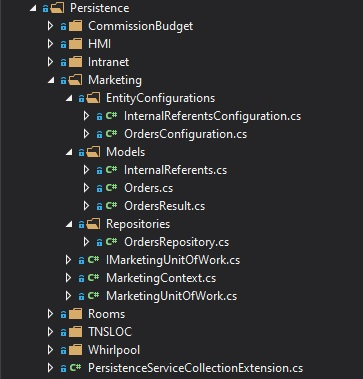
\includegraphics[width=8cm]{images/Persistence.jpg}\\
  \caption{Formato cartella persistence}\label{fig:persistence}
\end{center}
\end{figure}

Nella conformazione che si denota in figura~\ref{fig:persistence}, ciascuna cartella definisce un contesto applicativo di ed è articolata in:

\begin{itemize}
\item 
\textbf{Entity configurations:} vi sono le configurazioni delle entità presenti in \textbf{Models}, effettuando il mapping di tabelle e colonne nel database,
\item
\textbf{Models:} ciascun modello è un'entità che rappresenta l'analogo del record, o riga, di una tabella,
\item 
\textbf{Repositories:} volte all'interrogazione e manipolazione dati tramite l'uso di Data Manipulation Language (quali Linq e Nest, rispettivamente per database SQL ed ElasticSearch),
\item 
\textbf{IUnitOfWork:} interfaccia in cui vengono definite repository e metodo \verb|SaveChanges|,
\item
\textbf{DbContext:} in questa classe viene fornita la connection string del database (definita in \verb|appsettings|), si dichiarano i DbSet relativi ai model, che sono entity set utilizzati per le CRUD operations \cite{DbSet} ed in \verb|OnModelCreating| si applicano le configurazioni dei model,
\item 
\textbf{UnitOfWork:} implementa l'interfaccia creando la repository ed applicando il metodo \verb|SaveChanges| al context; quest'ultimo ha la funzione di salvare un insieme di modifiche in una transazione, oppure di eseguire un \textbf{rollback} (ossia un ripristino allo stato che precede l'aggiornamento)
\end{itemize}
\verb|PersistenceServiceCollectionExtension| si occupa di configurare le dependency injection per la creazione del context ElasticSearch.